\documentclass[tikz]{standalone}
\usepackage{pgfplots}
\pgfplotsset{compat=1.18}

\begin{document}

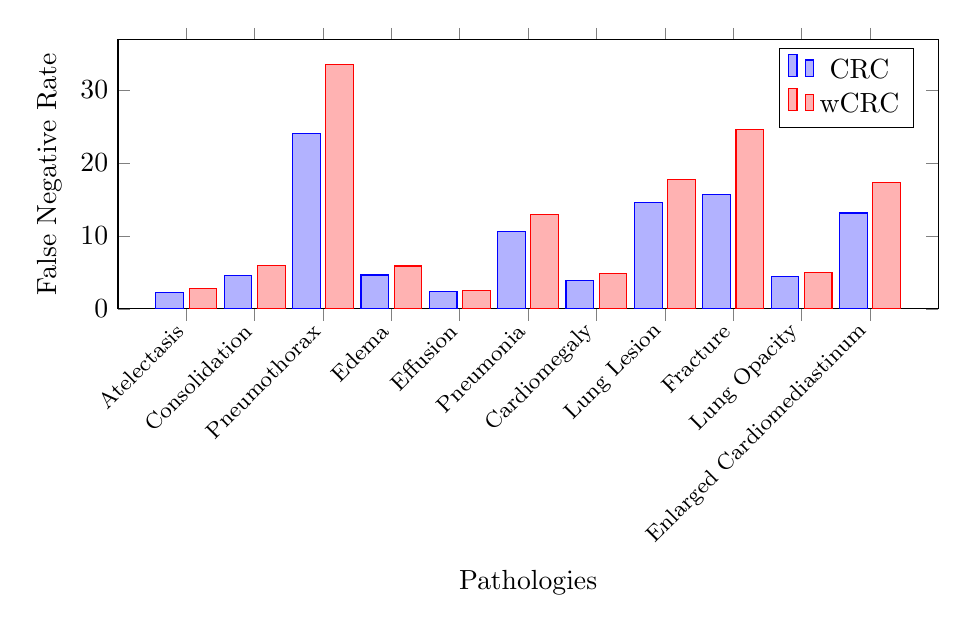
\begin{tikzpicture}
\begin{axis}[
    width=12cm,
    height=5cm,
    ybar,
    symbolic x coords={
        Atelectasis,
        Consolidation,
        Pneumothorax,
        Edema,
        Effusion,
        Pneumonia,
        Cardiomegaly,
        Lung Lesion,
        Fracture,
        Lung Opacity,
        Enlarged Cardiomediastinum
    },
    xtick=data,
    xticklabel style={
        font=\footnotesize,
        rotate=45,
        anchor=east
    },
    ymin=0,
    ylabel={False Negative Rate},
    xlabel={Pathologies},
    enlarge x limits=0.10,
    legend pos=north east,
]

\addplot coordinates {
    (Atelectasis, 2.2409)
    (Consolidation, 4.5714)
    (Pneumothorax, 24.0964)
    (Edema, 4.6436)
    (Effusion, 2.3545)
    (Pneumonia, 10.6667)
    (Cardiomegaly, 3.9258)
    (Lung Lesion, 14.6132)
    (Fracture, 15.7248)
    (Lung Opacity, 4.4635)
    (Enlarged Cardiomediastinum, 13.1524)
};
\addlegendentry{CRC}

\addplot coordinates {
    (Atelectasis, 2.8011)
    (Consolidation, 5.9048)
    (Pneumothorax, 33.5341)
    (Edema, 5.8855)
    (Effusion, 2.5257)
    (Pneumonia, 12.8889)
    (Cardiomegaly, 4.9073)
    (Lung Lesion, 17.7650)
    (Fracture, 24.5700)
    (Lung Opacity, 4.9364)
    (Enlarged Cardiomediastinum, 17.3278)
};
\addlegendentry{wCRC}


% \path (axis cs:{[normalized]1},0.9) coordinate (aux);
\end{axis}

% \draw[red, dashed] (current axis.east|-aux) -- (current axis.west|-aux) node [above right] {\(1 - \alpha\)};
\end{tikzpicture}

\end{document}
